% (c) 2017 Leonardo Aldegheri
% (c) 2017 Carlotta Gualtieri

\begin{comment}
\section{TODO}

\section{Esercizi}

\subsection{Esercizi dei singoli paragrafi}

\subsubsection*{\numnameref{sec:01_}}

\begin{esercizio}
\label{ese:D.19}
testo esercizio
\end{esercizio}

\begin{esercizio}\label{ese:03.1}
Consegna:
 \begin{enumeratea}
  \item  
 \end{enumeratea}
\end{esercizio}

\subsection{Esercizi riepilogativi}

\begin{esercizio}
\label{ese:D.19}
testo esercizio
\end{esercizio}

\begin{esercizio}\label{ese:03.1}
Consegna:
 \begin{enumeratea}
  \item  
 \end{enumeratea}
\end{esercizio}
\end{comment}

\section{Esercizi}
%label{}
  \subsection{Esercizi dei singoli paragrafi}
  %label{}
  \subsubsection*{1.1 Definizione di funzione}
  %label{}
  \begin{itemize}
  \item[1.1)] Riflettendo sulla definizione di 
funzione rispondi argomentando alle seguenti domande:
  \begin{itemize}
  \item[a)] Quali tra i 
seguenti oggetti, che puoi rappresentare sul piano cartesiano, è una 
funzione: circonferenza, ellisse, parabola con asse verticale?
  \item[b)] Quali tra i 
seguenti oggetti, che puoi rappresentare sul piano cartesiano, sono funzioni: 
retta verticale, retta orizzontale, retta obliqua?
  \item[c)] Considera una 
parabola con asse verticale e una con asse orizzontale, quale delle due è una 
funzione?
  \end{itemize}
  \item[1.2)] Determina il dominio delle 
seguenti funzioni
  \begin{itemize}
  \item[a)] $y= 4x^2+x+2$   
   \hfill  [ $D=R$ ]
  \item[b)] 
$y=\frac{3x+2}{x-5}$   \hfill   
   [ $D=R-\{5\}$ ]
  \item[c)] $y=\sqrt{9-x^2}   $ 
   \hfill   [ $D=[-3, 3]$ ]
  \item[d)] 
$y=\frac{4x}{\sqrt{x+2}}  $  \hfill   
   [ $D=]-2,+\infty[$ ]
  \item[e)] 
$y=\frac{2+3x}{x^2+7x+12}$   \hfill   
[$D=\mathbb{R}-\{-3,-4\}$]
  \item[f)] $y=e^{x+3}$\hfill   
   [$D=\mathbb{R}$]
  \item[g)] $y=\log_2(x+3)$  
\hfill  [$D=]-3, +\infty[$ ]
  \item [h)] $y=\ln(x^2+6x+8)$  
  \hfill   
[$D=]-\infty,-4[\cup]-2,+\infty[$]
  
\item[i)]$y=\frac{x^3+3x}{e^x+5}$\hfill   
  [$D=\mathbb{R}$]
  
\item[l)]$y=\frac{3x^2+4}{e^x-2}$   \hfill  
   [$D=\mathbb{R}-\{\ln2\}$]
  \item[m)] 
$y=\frac{4x-5}{2x-8}-\sqrt{x+3}$  \hfill  
[$D=[-3,4[\cup]4,+\infty[$]
  \item[n)]$y=\sqrt{\log(x+4)}$ 
   \hfill  [$D=[-3,+\infty[$]
  \item[o)]$y=(x+5)^{x+3}$  
   \hfill  [$D=]-5,+\infty[$]
  \item[p)] 
$y=2\sin{x}+\cos{2x}$   \hfill   
[$D=\mathbb{R}$]
  
\item[q)]$y={2+\cos{3x}}{2\sin{x}}$   \hfill  
   [$D=\mathbb{R}-\{k\pi,\,k\in \mathbb{Z}\}$]
  \item[r)] $y=\arcsin(x+2)$  
   \hfill  [$D=[-3, -1]$]
  
\item[s)]$y=\arctan(\frac{3}{x+2}) $  \hfill  
   [$D=\mathbb{R}-\{-2\}$ ]\\

  \end{itemize}

\newpage
  
  \item[1.3)] Dall'analisi visiva del grafico deduci il 
dominio e codominio della funzione.
  \begin{figure}[htpb!]
  \centering

% \begin{minipage}{.49 \textwidth}
% \end{minipage}
% \hfill
% \begin{minipage}{.49 \textwidth}
% \end{minipage}

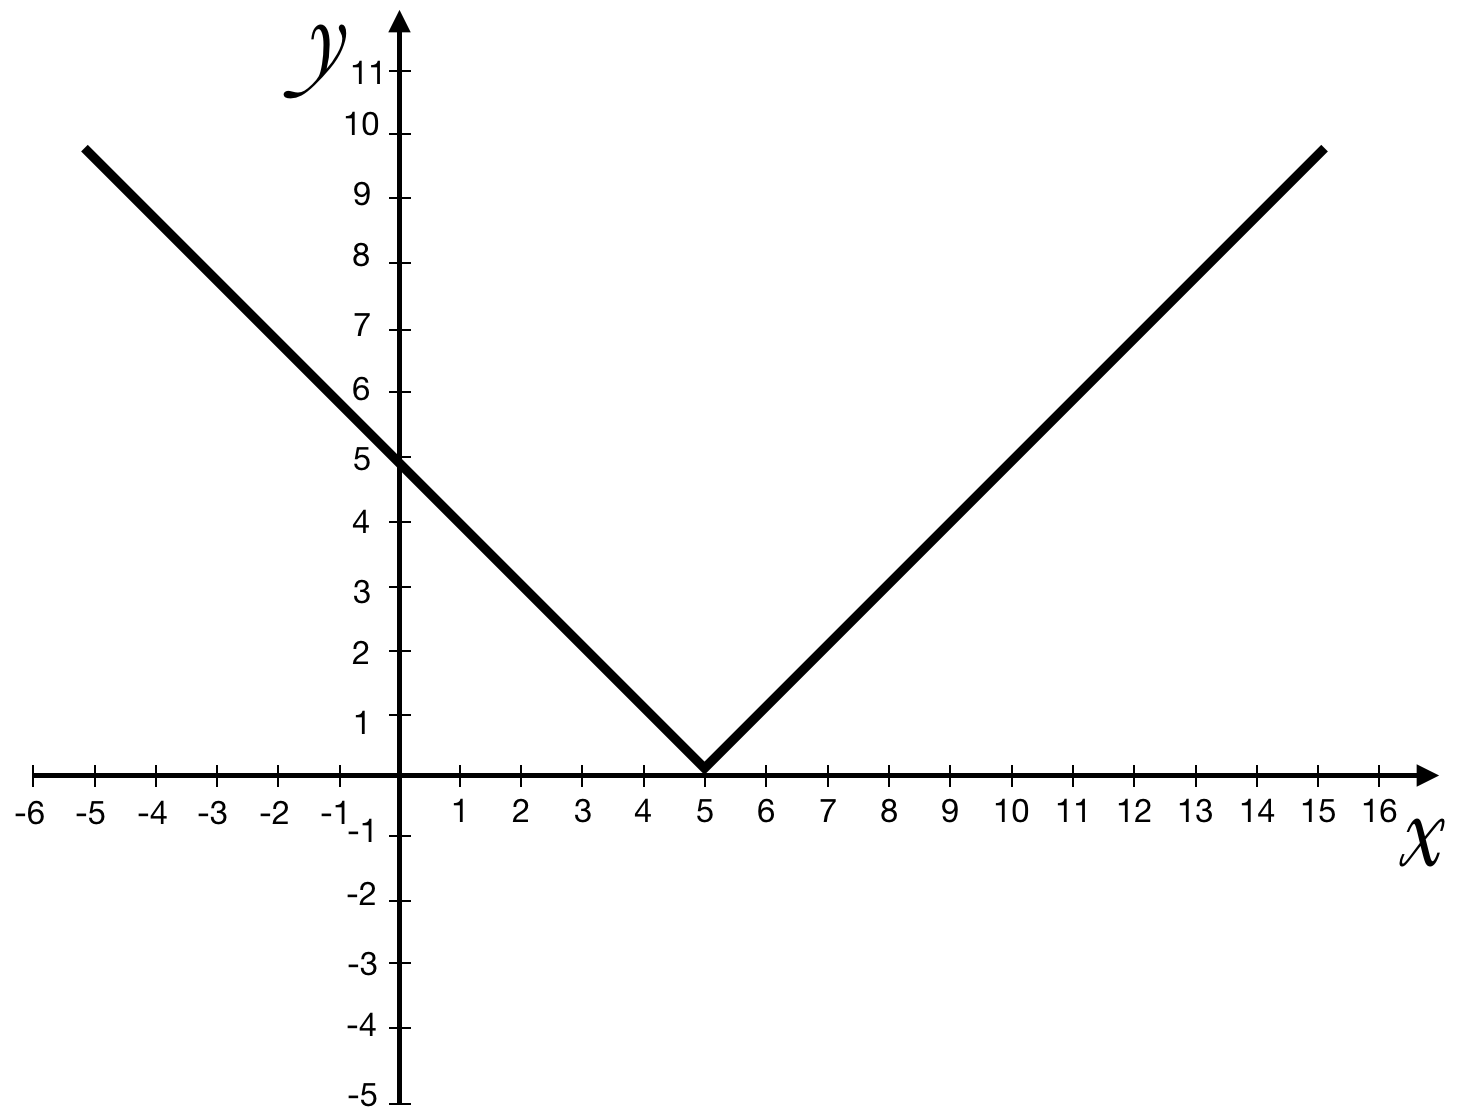
\includegraphics[width=0.45\textwidth]{img/funz_16.png} \quad 
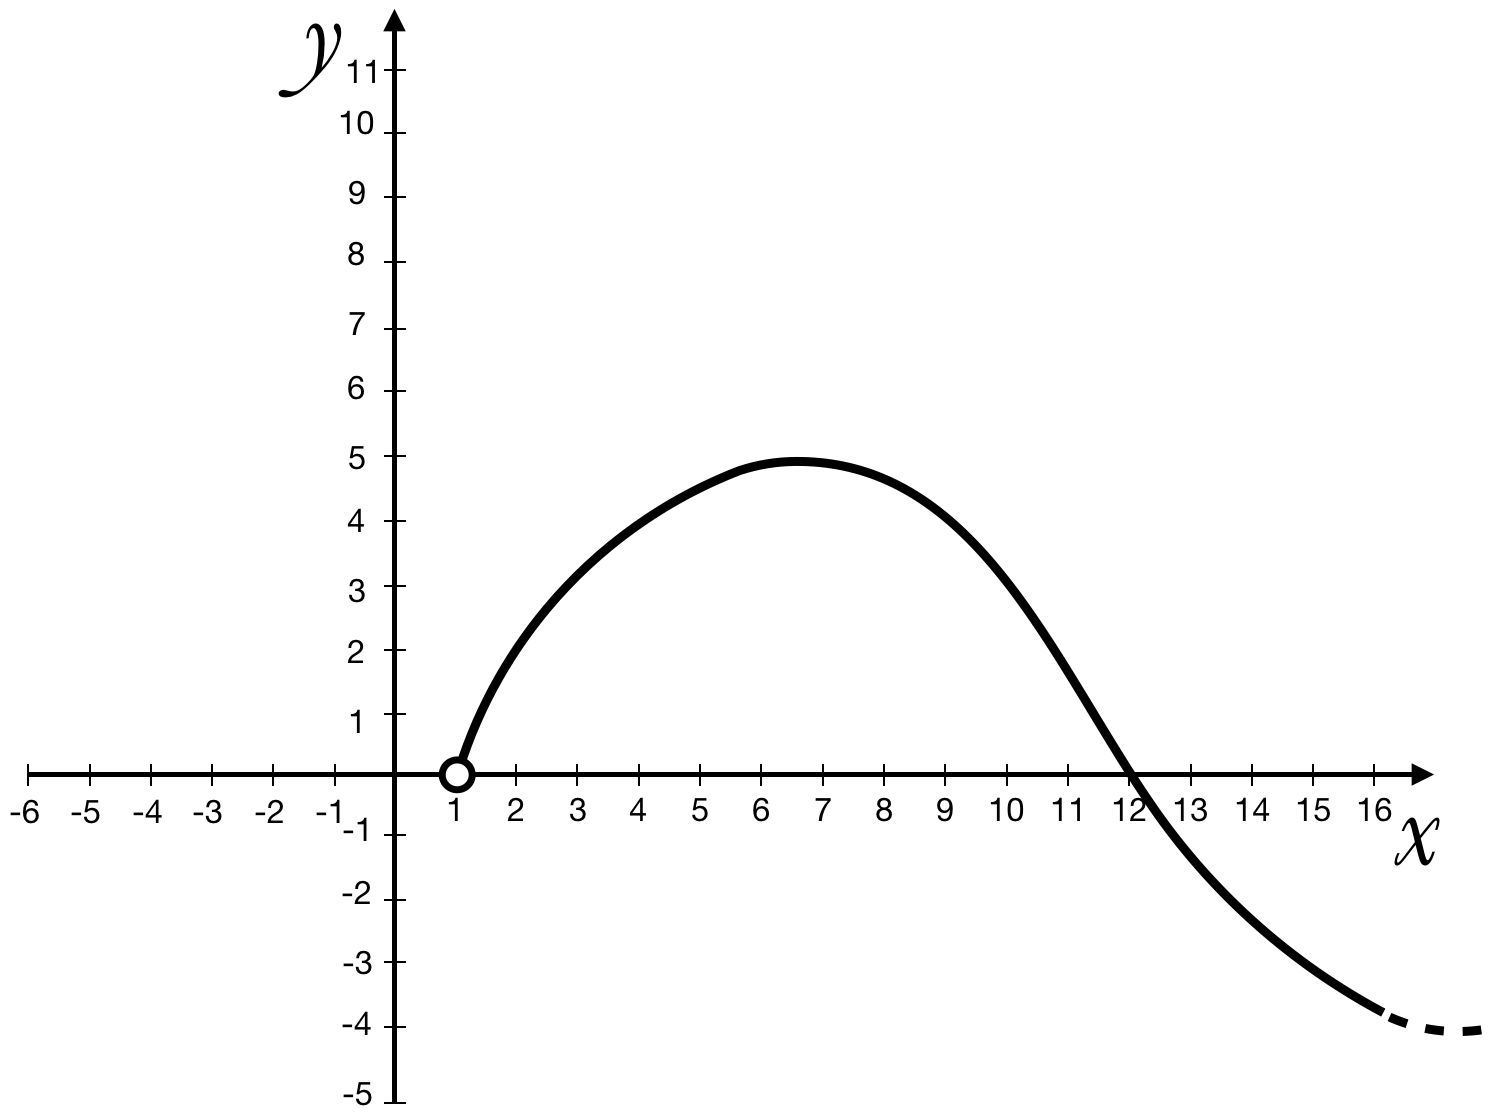
\includegraphics[width=0.5\textwidth]{img/funz_17.png}  
  
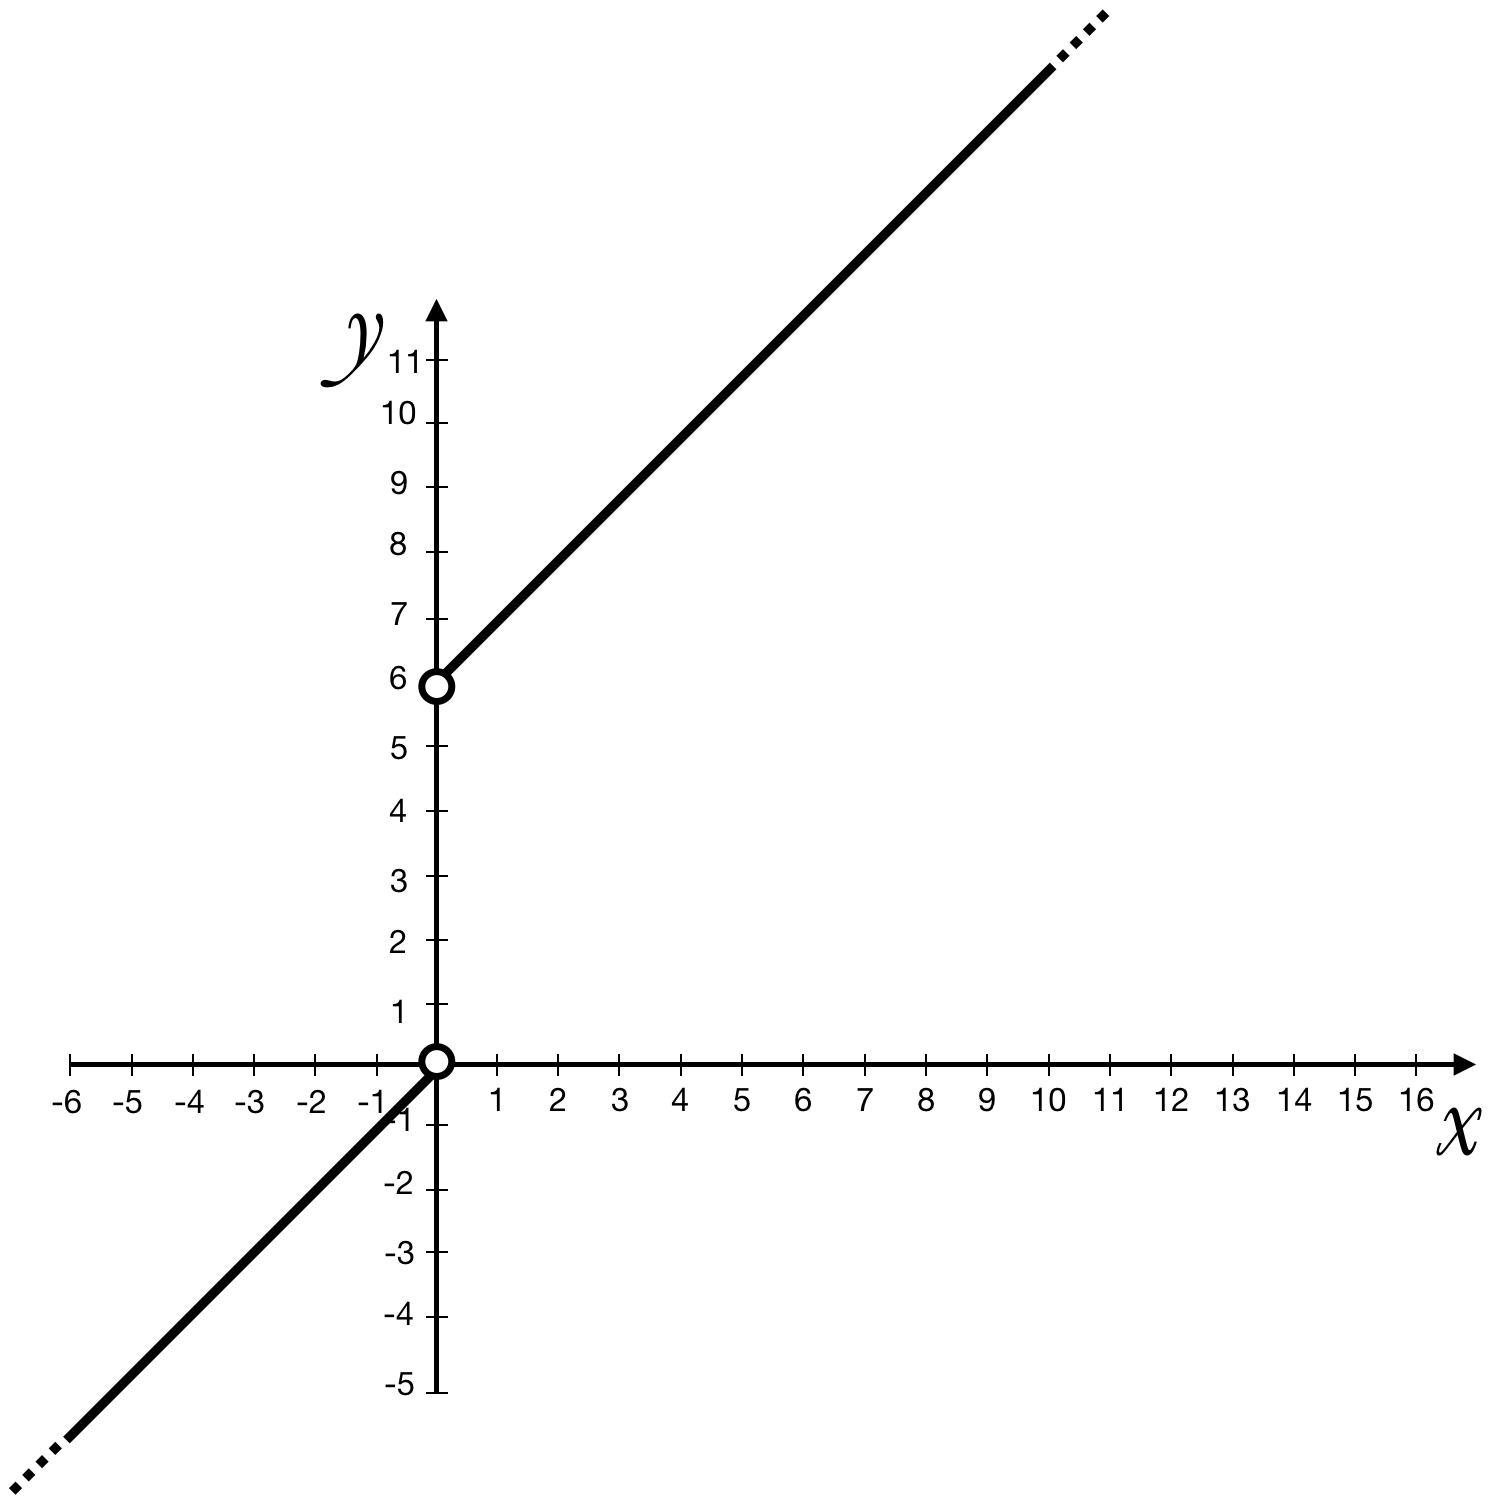
\includegraphics[width=0.45\textwidth]{img/funz_17a.png} \quad
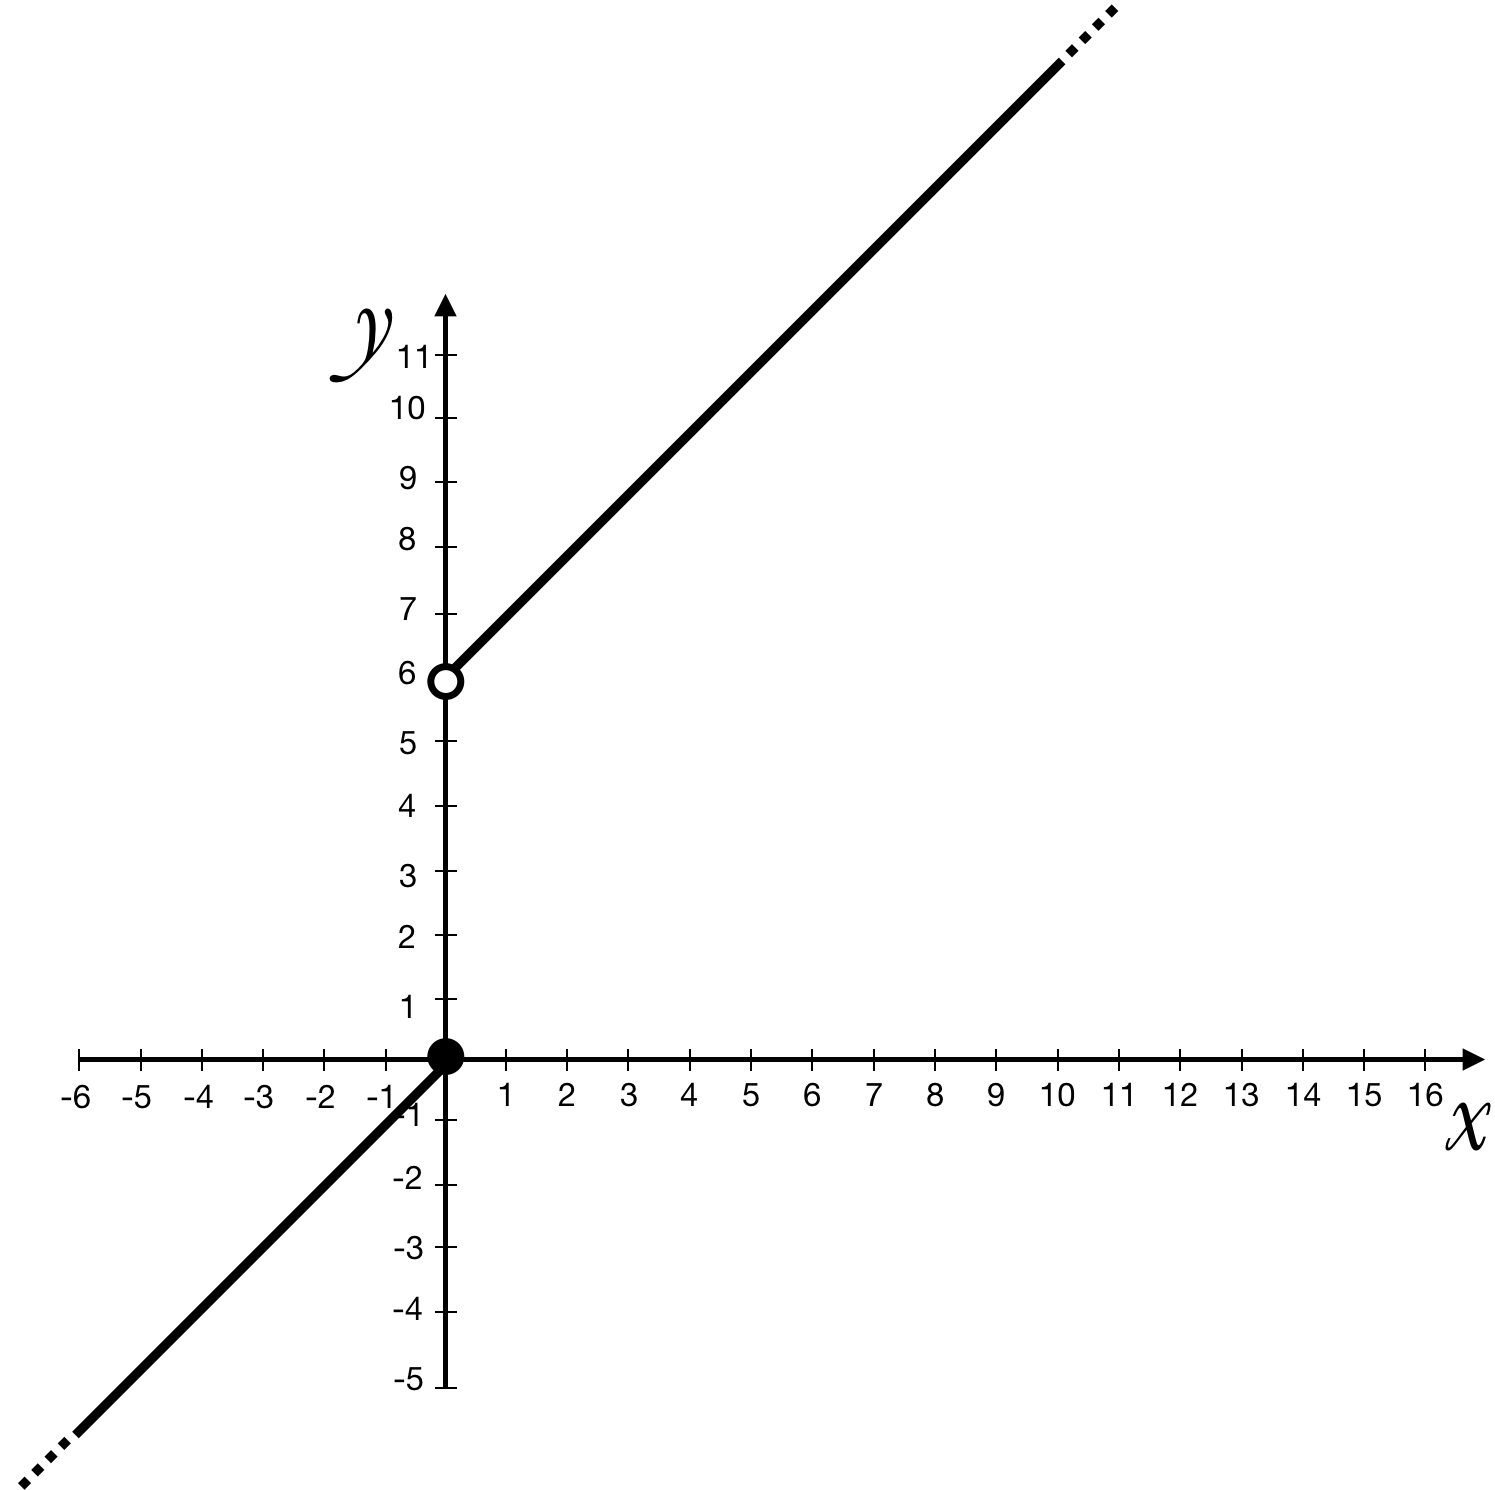
\includegraphics[width=0.45\textwidth]{img/funz_17b.png}   
  
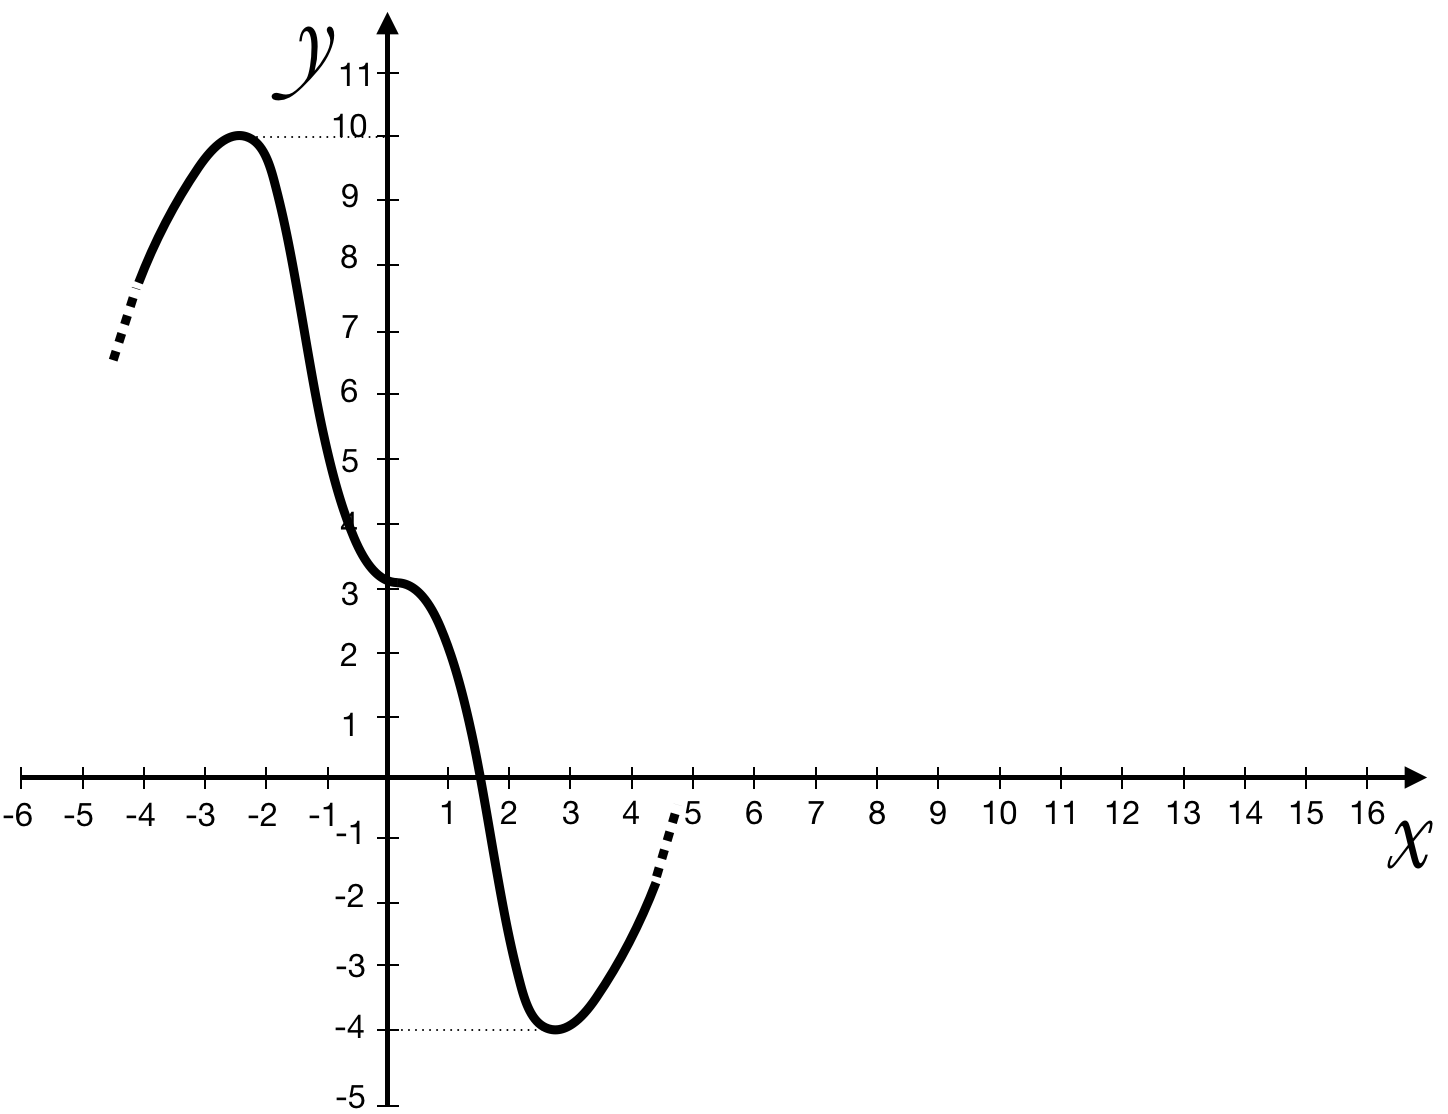
\includegraphics[width=0.45\textwidth]{img/funz_17c.png} \quad
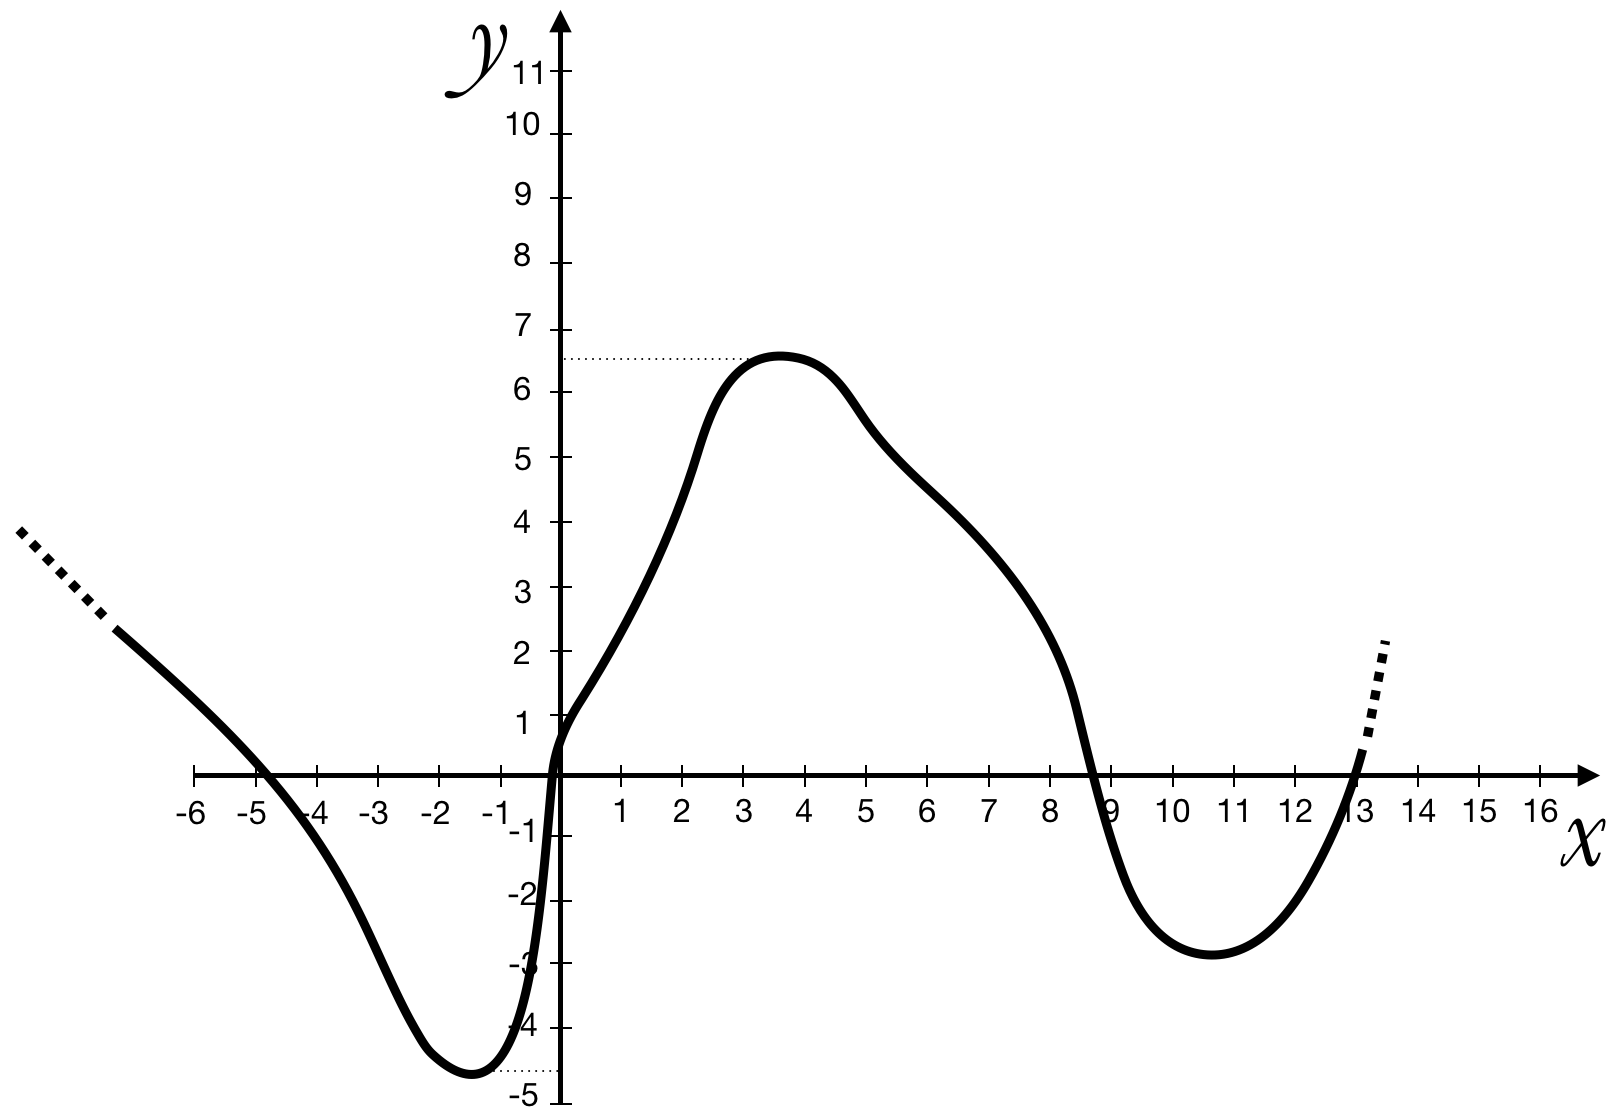
\includegraphics[width=0.45\textwidth]{img/funz_17d.png}
  %\caption{}
  %\label{fig:funz_14abc}
  \end{figure}
  \end{itemize}

\newpage

\subsubsection*{1.2 La rappresentazione di una funzione}
%label{}
\begin{itemize}
  \item[1.4)] Immagina l'evoluzione della temperatura ora per ora nella 
città di Firenze, in una giornata di agosto, costruiscine la rappresentazione 
tabulare e quella grafica.
  \item[1.5)] Rappresenta graficamente le seguenti funzioni:
  \begin{itemize}
  \item[a)] $y=\sin2x$
  \item[b)] $y=3x+2$
  \item[c)] $y=x^2+2$
  \item[d)] $y=x^2+2x+3$
  \item[e)] $y=\log{(x+1)}$
  \item[f)] $y=e^x+2$
  \item[g)] $y=\frac{x+2}{2x-4}$
  \item[h)] $y=\sqrt{9-x}$
  \item[i)] $y=\sqrt{9-4x^2}$
  \item[l)] $y=\sqrt[3]{x}$
  \item[m)] $y=\vert x^2+4x+3\vert$
  \end{itemize}
\end{itemize}

\subsubsection*{1.3 Le proprietà di una funzione}
%label{}
\begin{itemize}
  \item[1.6)] Stabilisci se le seguenti funzioni, rappresentate 
graficamente, sono iniettive, suriettive o biunivoce, motivando la risposta.
  \begin{multicols}{2} 
  \begin{itemize}
  \item[(a)] $f:\mathbb{R}\to[0,+\infty[$
  \item[(c)] $f:\mathbb{R}\to]0,+\infty[$
  \item[(b)] $f:\mathbb{R}\to\mathbb{R}$
  \item[(d)] $f:\mathbb{R}\to\mathbb{R}$
  \end{itemize}
  \end{multicols}
  
  \begin{figure}[htpb!]
  \centering
  
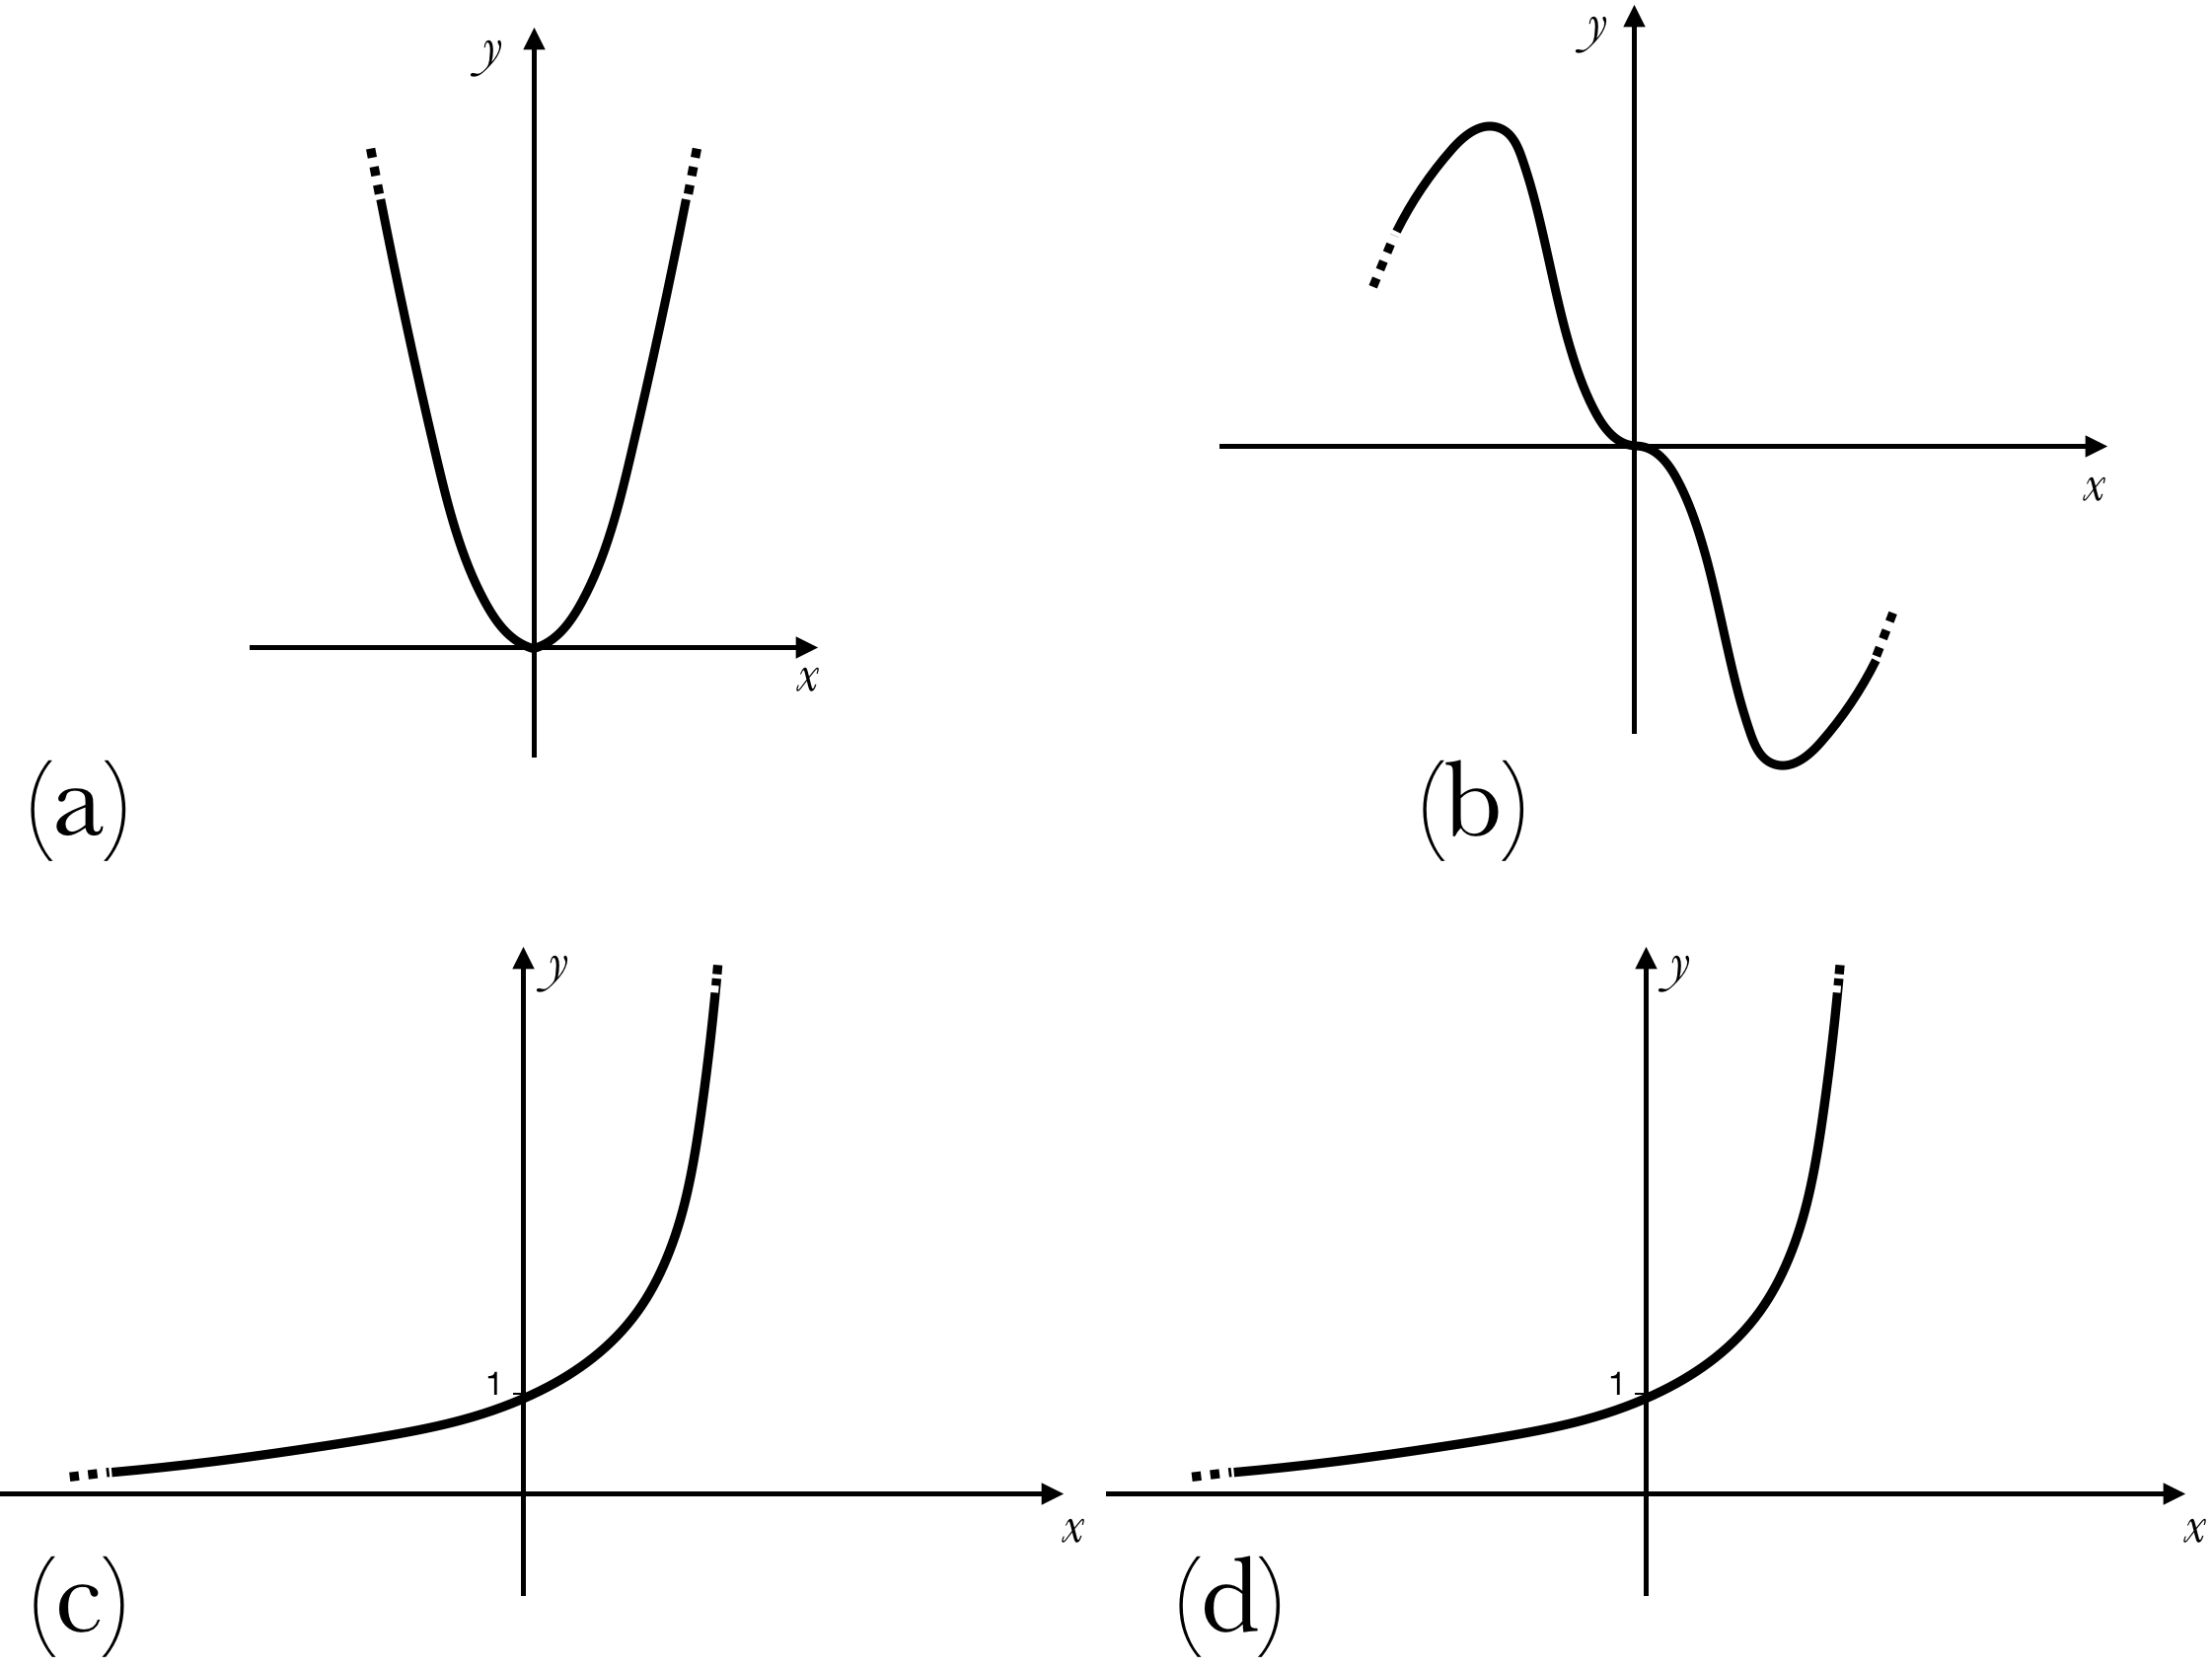
\includegraphics[width=0.65\textwidth]{img/funz_18.png}%\caption{}
  %\label{fig:funz_14abc}
  \end{figure}
\end{itemize}
\subsubsection*{1.4 Le caratteristiche di una funzione}
%label{}
\begin{itemize}
  \item[1.7)] Verifica se le seguenti funzioni sono pari o dispari.
  \begin{itemize}
  \item[a)] $y=2x+3$   \hfill   
  [né pari né dispari]
  \item[b)] $y=x^3+x$   \hfill  
   [dispari]
  \item[c)] $y=\frac{x^2+3}{x}$   \hfill  
  [dispari]
  \item[d)] $y=\frac{3x^4}{2+x^2} $   \hfill  
   [pari]
  \item[e)] $y=\tan{x}+\sin{x} $   \hfill   
 [dispari]
  \item[f)] $y= \log{(x-1)}$   \hfill   
[né pari né dispari]
  \end{itemize}
  
  \item[1.8)] Stabilisci se le seguenti funzioni sono periodiche, 
individuandone l'eventuale periodo.
  \begin{itemize}
  \item[a)] $y=\sin4x$   \hfill   
  [periodica $T=\frac{\pi}{2}$]
  \item[b)] $y=\tan2x$   \hfill   
  [periodica $T=\frac{\pi}{2}$]
  \item[c)] $y=\cos3x+1$   \hfill   
   [periodica $T=\frac{2\pi}{3}$]
  \item[d)] $y=\cos x+x $   \hfill  
   [non periodica]
  \item[e)] $y=\tan{\frac{x}{5}} $   \hfill   
   [periodica $T=5\pi$]
  \item[f)] $y= \sin(x+1)$   \hfill   
[periodica $T=2\pi$]
  \item[g)] $y= \sin x+1$   \hfill   
[periodica $T=2\pi$]
  \item[h)] $y= \sin x+x$   \hfill   
[non periodica]
  \item[i)] $y= \sin{\frac{x}{4}}$   \hfill   
  [periodica $T=8\pi$]
  \item[l)] $y= 2^{\sin{x}}$   \hfill   
[periodica $T=2\pi$]
  \item[m)] $y=x\cos x$   \hfill   [non 
periodica]
  \end{itemize}
\end{itemize}

\subsubsection*{1.5 La classificazione delle funzioni}
\begin{itemize}
  \item[1.9)] Classifica prima riguardo alle categorie algebrico o 
trascendente e poi rispetto alle categorie fratta o intera e razionale o 
irrazionale le seguenti funzioni.
  \begin{itemize}
  \item[a)] $y=\frac{x^2+x+2}{3x}$
  \item[b)] $y=\frac{4}{\sqrt{x-6}}$
  \item[c)] $y=e^x+x$; $y=\sqrt[3]{x^2+x}$
  \item[d)] $y=\frac{1}{3}\sqrt{3-x}$
  \item[e)] $y=\frac{\sin x}{4}$
  \item[f)] $y=\frac{x^2-4x}{3+\sqrt{2}}$
  \end{itemize}
\end{itemize}

\subsubsection*{1.6 Funzioni inverse, composte e uguali}
%label{}
\begin{itemize}
  \item[1.10)] Stabilisci se le seguenti funzioni sono invertibili 
senza restrizioni, giustificando la risposta.  \begin{itemize}
  \item[a)] $y=2x+3$ \hfill [invertibile]
  \item[b)] $y=x^2+9x+18$ \hfill [non invertibile]
  \item[c)] $y=e^x$ \hfill [invertibile]
  \item[d)] $y=\ln{x}$ \hfill [invertibile]
  \item[e)] $y=x^3+3x^2+x$ \hfill [non invertibile]
  \item[f)] $y=\sin x$ \hfill [non invertibile]
  \end{itemize}
  
  \item[1.11)] Determina l'inversa della funzione data, specificando il 
suo dominio.  
  \begin{itemize}
  \item[a)] $y=4x+3$ \hfill [$y=\frac{x-3}{4},\, 
D=\mathbb{R}$]
  \item[b)] $y=e^{2x}$ \hfill [$y=\frac{\ln x}{2},\, 
D=]0,+\infty[$]
  \item[c)] $y=x+1$ \hfill [$y=x-1,\, D=\mathbb{R}$]
  \item[d)] $y=\ln(x+1)$ \hfill [$y=e^x-1,\, 
D=\mathbb{R}$]
  \end{itemize}
  
  
  \item[1.12)] Date le funzioni $f(x)$ e $g(x)$ determina le 
espressioni analitiche di $f\circ g$ e di $g\circ f$.% non riesco a rendere 
ben leggibile questo esercizio
  \begin{itemize}
  \item[a)] $f(x)=\sqrt[3]{x+3}$  \\  $g(x)=\log_4{x}$  
\\  \hfill   $[(f\circ g)(x)=\sqrt[3]{\log_4{x+3}}; (g\circ 
f)(x)=\log_4{(\sqrt[3]{x+3})}]$
  
  \item[b)] $f(x)=3^x$  \\ $g(x)=x-5$   \\   
\hfill  $[(f\circ g)(x)=3^{x-5}; (g\circ f)(x)=3^x-5]$
  
  \item[c)] $f(x)=\cos3x$  \\ $g(x)=\sqrt{x^2+3}$  \\ 
   \hfill  $[(f\circ g)(x)=\cos{3\sqrt{x^2+3}}; (g\circ 
f)(x)=\sqrt{(\cos{3x})^2+3}]$
  
  \item[d)] $f(x)=x^2+3$ \\  $g(x)=2x+1$  \\  
\hfill  $[(f\circ g)(x)=(2x+1)^2+3=4x^2+4x+4; (g\circ 
f)(x)=2(x^2+3)+1=2x^2+7]$
  \end{itemize}
\end{itemize}
%mancano esercizi su limitatezza e monotonia (provvedo a creare dei grafici e 
% semmai si aggiungono nei prossimi giorni...










